\chapter{Research Proposal}
\label{chap:proposal}

% feasible
% appropriate:  likely to deliver the evidence needed to answer the question
% rigorous
% likely to deliver valid, reliable, (generalisable?) results
% ethical
% justified


% \section{Justification} <-- already Chapter 2 and 3 contain it


% motivation
% Our goal is to provide a tool for doing framing analysis of multiple articles about a certain event, to highlight the different framing techniques and compare the resulting articles.
In this chapter, we present an overall description of the framework we want to build in order to highlight the different framing techniques and compare the articles that different sources create around a single event.
% This needs to be taken as a description of the requirements
% This description of the framework acts as a wireframe, where specific choices will be done based on evidence, 
As we can see in Figure~\ref{fig:diagram}, we are taking the research questions and sub-questions from the previous chapter, and for each one of them we have a process that from the hypothesis leads to some outputs using a separate and distinct analysis.

% outline
The structure of this chapter follows the columns that represent the different research questions.

\begin{figure}[!htb]
    \centering
    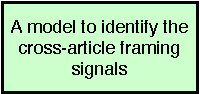
\includegraphics[width=\linewidth]{figures/diagram-RQ.pdf}
    \caption{The relationships between the research questions and the evaluations.}
    \label{fig:diagram}
\end{figure}

% Each one of the vertical columns is described in a different section below.

% This chapters begins with Section~\ref{sec:prop_pipeline} that outlines how we want to take existing works from the framing and similarity research areas.
% Then in Section~\ref{sec:prop_rq1} we target RQ1, giving some insights about some new analysis that we can do that would extend the existing automated framing analysis.
% And then in Section~\ref{sec:prop_rq2} we explain how we can analyse the role of news sources, for the relationship between their alignment and the framing they apply and how the stories are changed over time.



\section{Cross-article framing analysis (RQ1)}
\label{sec:prop_rq1}

% RQ1: framing differences
To address the first Research Question
\textbf{(How can we automatically reveal the framing differences in articles presenting the same event?)}, we aim to resolve two sub-questions separately: the first one analyses the \emph{importance} for the reader of comparing multiple articles to understand the framing that is being applied on the news through the revelation of specific framing signals, and the second one explores \emph{how} we can build a tool to identify these framing signals automatically.
In other words, while the first sub-question deals with the importance for the readers, the second question instead targets the automated detection.
The dependency between the two sub-questions underlines that the second column needs the outputs of the first one to know how to label the framing differences.

% we aim to automatically identify \textit{signals of framing} that otherwise would not be noticeable: differences in emphasis and selection of details.
% These signals, while they are defined in the theoretical works, they have not been targeted in the automatic framing analysis.

% Starting with the \textit{emphasis}, we aim to analyse how different articles give importance to specific details.
% While existing works just focus on the usage of loaded terms and repetitions to indicate the presence of emphasis, we can enrich this analysis by seeing how other articles describe the same event.
% Comparing between different articles we can spot differences in the main focus of the article (e.g., the title is an indicator) or look at how the details are presented in a different order to set the priorities for the reader.
% And this can be combined with loaded language analysis, to see how certain details are emphasised and pushed with specific words in very different ways.
% \todo{figure}

% To understand the \textit{selection of details} instead, the idea is to compare the articles and get the common, unique and omitted pieces~\cite{bountouridis2018explaining} and then use some linguistic features (e.g., subjectivity, framing devices) to understand what is their role, may them be full sentences or just specific words that have been added or removed strategically.
% With this analysis, we aim to provide for each article, multiple sides of the same story with an insight into what changes between them.


\subsection{The usefulness of multiple articles (RQ1.1)}
% RQ 1.1: cross-article signals
The first column represents a line of research that is needed to understand how useful is for readers to confront the information available in multiple articles to spot the framing techniques used.
% signals
In order to describe and characterise the framing we started from the literature review to gather concrete manifestations of framing, both in theoretical works and in detection methods.
As we have seen in subsection~\ref{ssec:lit_framing_theory}, different manifestations have been theorised and studied in practical studies
% what we mean by signal
We name these manifestation \emph{signals} because they are signalling the presence of the framing, which is a abstract concept, but they are tangible and can be seen as concrete features.
For example, loaded language can be seen as a signal that can be observed on specific words that have a strong sentiment, and evokes frames of strength, violence, threat and similar.
Or the strategic omission or inclusion of certain details that have the role of shifting the opinion of the reader.
What we want to investigate is whether we can ease their detection by comparing multiple articles, 
% extend this set of signals by exiting the limitations of a single-article analysis. 
and therefore the specific sub-question is \textbf{What is the contribution of comparing multiple articles to reveal signals of framing?}

% Hypothesis
Our hypothesis is that having multiple articles would allow users to easier detect the framing signals that they are faced with, especially with some of them that are particularly subtle to reveal when just looking at a single article at a time.
% these signals will reveal far more than the single-article framing analysis.
As we described in a position paper~\cite{mensio2020towards}, such signals vary from differences in the emphasis (e.g., different articles focus their headlines on a different detail, or present the story in a different order) to the selection of details (e.g., some articles may decide to omit some parts of the story that is reported by others, or include unnecessary details to push for a certain narrative) or also to different term choices (e.g., being stronger in the language, or evoke specific feelings or related events).
For this reason, we want to test how important it is to see multiple articles that treat the same event to discover their point of view/framing through the signals used in the text.

% % This is is the starting point to identify the differences, with a contrastive analysis. We propose here a set of  that can bring the narrative analysis a step further:
% \begin{itemize}
%     \item The \textbf{main focus} of the compared articles is on a different part or detail of the story: this means that while they are both describing the same broad event, they are trying to emphasise or prioritise two different aspects.
%     % Prioritisation is usually based on negativity / unexpectedness / superlativeness \cite{zahid2019towards}.
%     This signal can be computed by looking at the most similar sentence to the article title (proxy of the emphasis), and seeing how it is represented in other documents.
%     % Two articles that are semantically similar overall (they also have sentence-sentence pairs very similar) focus on different details when the titles are similar to different sentence-level cliques.
    
%     \item \textbf{Ordering}: the compared articles present the same details, but in a different order.
%     Re-ordering events tends to be an efficient way of creating implicit cause-effect relationships. 
%     To do this comparison, it is sufficient to find the crossovers in the sentence-level connections.

%     \item \textbf{Selection of details}:
%     One article is \emph{omitting} certain details that have been reported by other articles, or is describing events that are \emph{corroborated} by other sources, or has \emph{unique parts} that do not occur in other articles~\cite{bountouridis2018explaining}.
%     In addition to seeing which parts are selected or omitted, the narrative analysis can help us to find some insights about them (e.g., the article is omitting subjective statements reported by others, or is describing a background event that others did not include).
%     % For the detection of this case, we rely on the work~\cite{bountouridis2018explaining}.
    
%     \item The articles are \textbf{framing} the narrative in different ways from each other. This manifests through comparing linked sentences to observe the differences in terms of framing features: the considered articles are describing the same events but with different framing and reasoning.
%     One concrete example is the usage of \emph{causality}: one article may contain causality signposting between a pair of sentences that is absent elsewhere.
%     % \item The article uses \textbf{causality as a weapon} (where there is no proof of causality).
%     % An article is expressing causality when there are certain devices (signposting) between two sentences/events.
%     % Different articles may show the causality with different levels, so one sees it as causal and the other one does not link the events.
%     Or as another example, the usage of \emph{specific words} can reveal a specific framing: talking about the same detail or entity, the usage of verbs or adjectives may change.
%     % find strong sentiment and subjective words 
%     % (as adjectives for the same entity, or as verbs).
%     % Detail (e.g. black man instead of just saying man, to add a subtle bias).
%     For detecting such peculiarities, %and comparing them, we can combine the framing signals with 
%     features as Named Entities and subjectivity may be combined.
%     % use features coming from subjective and sentiment analysis.

%     \item The comparison can be also done on the \textbf{subjectivity} of the article: both at the document level (saying that this is an opinion piece, while a similar one is more factual) or at the sentence level, by interweaving this signal with the ones proposed before.
%     % is a \textbf{mix of factual and opinionated / subjective} content: subjectivity values on the full document and on specific sentences.
%     % A sentence is on one article subjective and a similar one on a different article is objective.
%     % Also look at the role of the sentence (commentary, action, background). 

% \end{itemize}

% From the signals in Figure~\ref{fig:comparison}, we can see that the first article pushes the narrative towards \texttt{risk} and other negative frames, to sustain the idea presented in the title ``Britain on Edge''.
% The second article, even though it has a lot of information in common with the first one, is more confident on the preparedness of the National Health Service to face the virus (e.g., \texttt{confidence}, \texttt{expertise}).
% The extraction of these cross-article signals is the first step to finding possible cases of manipulation.

% The expansion and refinement of these signals will help us answer RQ1.1.


% analysis
In order to validate our hypothesis, we will run a \textbf{user study} where participants will be shown different articles that present the same event with some differences.
To test the hypothesis of framing being easier to spot when multiple articles are available, we plan to first present to the user just one article and ask to find the framing signals. Then we show also the second article on the side with different details and ask again.
In both the steps, the input asked from the user is to highlight parts of the article(s) and to say why it is providing a certain view angle, as a free text. To obtain these annotation, users will first be shown with the framing techniques identified in the literature, to understand what they are looking for.
We will then compare the number and type of annotations coming from the two different situations (one singe article or multiple articles).
It is important to divide the annotators of a certain pair of articles in two sub-groups in order to divide the effect of ``seeing again the same article twice'' (unwanted) from ``seeing the article compared to another one'' (wanted). For this reason, if we consider A1 and A2, user U1 will first see A1 then A1+A2, while U2 will first see A2 then A1+A2. In this way we can sum CA1(before)+CA2 for U1 and CA1+CA2(before) for U2 where each observation is done at first sight of the corresponding article (see Figure~\ref{fig:user_study}).

% Hypothesis: users will be able to see more signals in the second phase.

\begin{figure}[!htb]
    \centering
    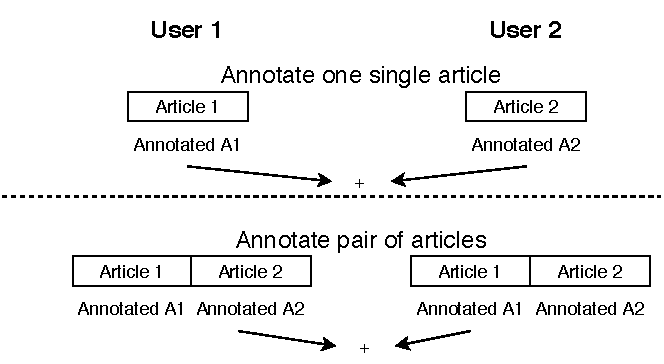
\includegraphics[width=\linewidth]{figures/diagram-user-study-flow.pdf}
    \caption{How to compare the user annotations to exclude effects of second-reading}
    \label{fig:user_study}
\end{figure}
\todo{improve figure to represent better the user study (e.g., annotated pair of articles)}


% requirements
% data (hand-picked samples from sources with different political alignment)
The pairs of articles to be shown will come from a selected subset from clusters of documents that are presenting the same detail, with some differences in the terms used. For this reason they need to be revised and checked.
The clusters will come from articles suggested by AllSides and other news aggregators like Google News, testing both differences from opposite political views as well as articles without any difference in the political bias.
To identify the pairs of documents we plan to use the help from similarity models that, as will be seen in Chapter~\ref{chap:plan}, have been investigated and used to cluster documents and sentences.

% Participants will be presented with two articles and will be asked a set of questions that investigate the effect of having different terms, different details and how user think this is related to try to push for a certain perspective on the events described.

% Do the articles have the same point of view? Do they convey the same message? Title? Details?
% Sentences
% - Do these sentences have different information?
% - Do they provide different perspective?
% - Are there any terms that push for a certain perspective?
% - What is the difference in the intent of communication?
%   - Detail (random, look like professional and detailed, mislead, emphasise on something)
%   - Word choice: emphasise, promote, demote
% if they value the selected differences as signals of the different point of view of the sources (framing), and what they think that the difference is (is it that they are omitting something, commenting, emphasising, other)?

% Or study 2 (better):


% outputs
The annotations will be manually examined with two goals.
First, to see if the annotators (using inter-annotator agreement measures) are able to spot more signals when they have different articles available.
This will prove or disprove our hypothesis that framing can be revealed easier in this setting.
And second, the annotations will be revised manually to bring them back to some categories that represent framing signals. An example could be ``omission of opposing detail'' or ``biased term''. We need to come up with a set of labels that we can assign to the differences pointed out by the users, guided by their descriptions.



\subsection{Automated framing detection (RQ1.2)}
% how would a cross-article framing analysis perform

The second part of the first Research Question requires building and evaluating an automated method to extract the signals identified in the first user study.
Unlike traditional methods of frame detection that mainly rely on extracting features from single articles to build a classification model, we want to use external features that come from the comparison of multiple articles. Such features could be the uniqueness of certain details (sentences or words) when comparing to other articles describing the same event, or including similar words that are used as substitutes in other articles.
The sub-question we address is the following:
\textbf{To what extent can we automatically recognise framing signals using information from multiple documents?}
% Previous research has been focusing on some of the signals, which we can consider as

% implementation
To implement a method that exploits the differences between multiple articles, we need to be able to use the similarities and differences between the considered documents.
For this reason, we plan to rely on the approaches described in the Literature Review~\ref{sec:lit_relationships} where we analysed some methods that are able to find the similarities at different granularities, and expose the differences of the details provided.
% Based on the initial experiments done to see the similarity between documents, we are implementing a processing pipeline that is able to retrieve, process and compare articles.
The step of feature extraction will be based on a pipeline that will process the documents in several steps
\todo{pipeline description in short}
% how to build on top of the cross-article representation
How the outputs of the pipeline can be used for detecting and navigating relationships.
For the detection of the signals, involve reasoning over the features already provided by the pipeline and building a model that provides as outputs span annotations of framing that will say which framing technique has been used.

\begin{figure}[!htb]
    \centering
    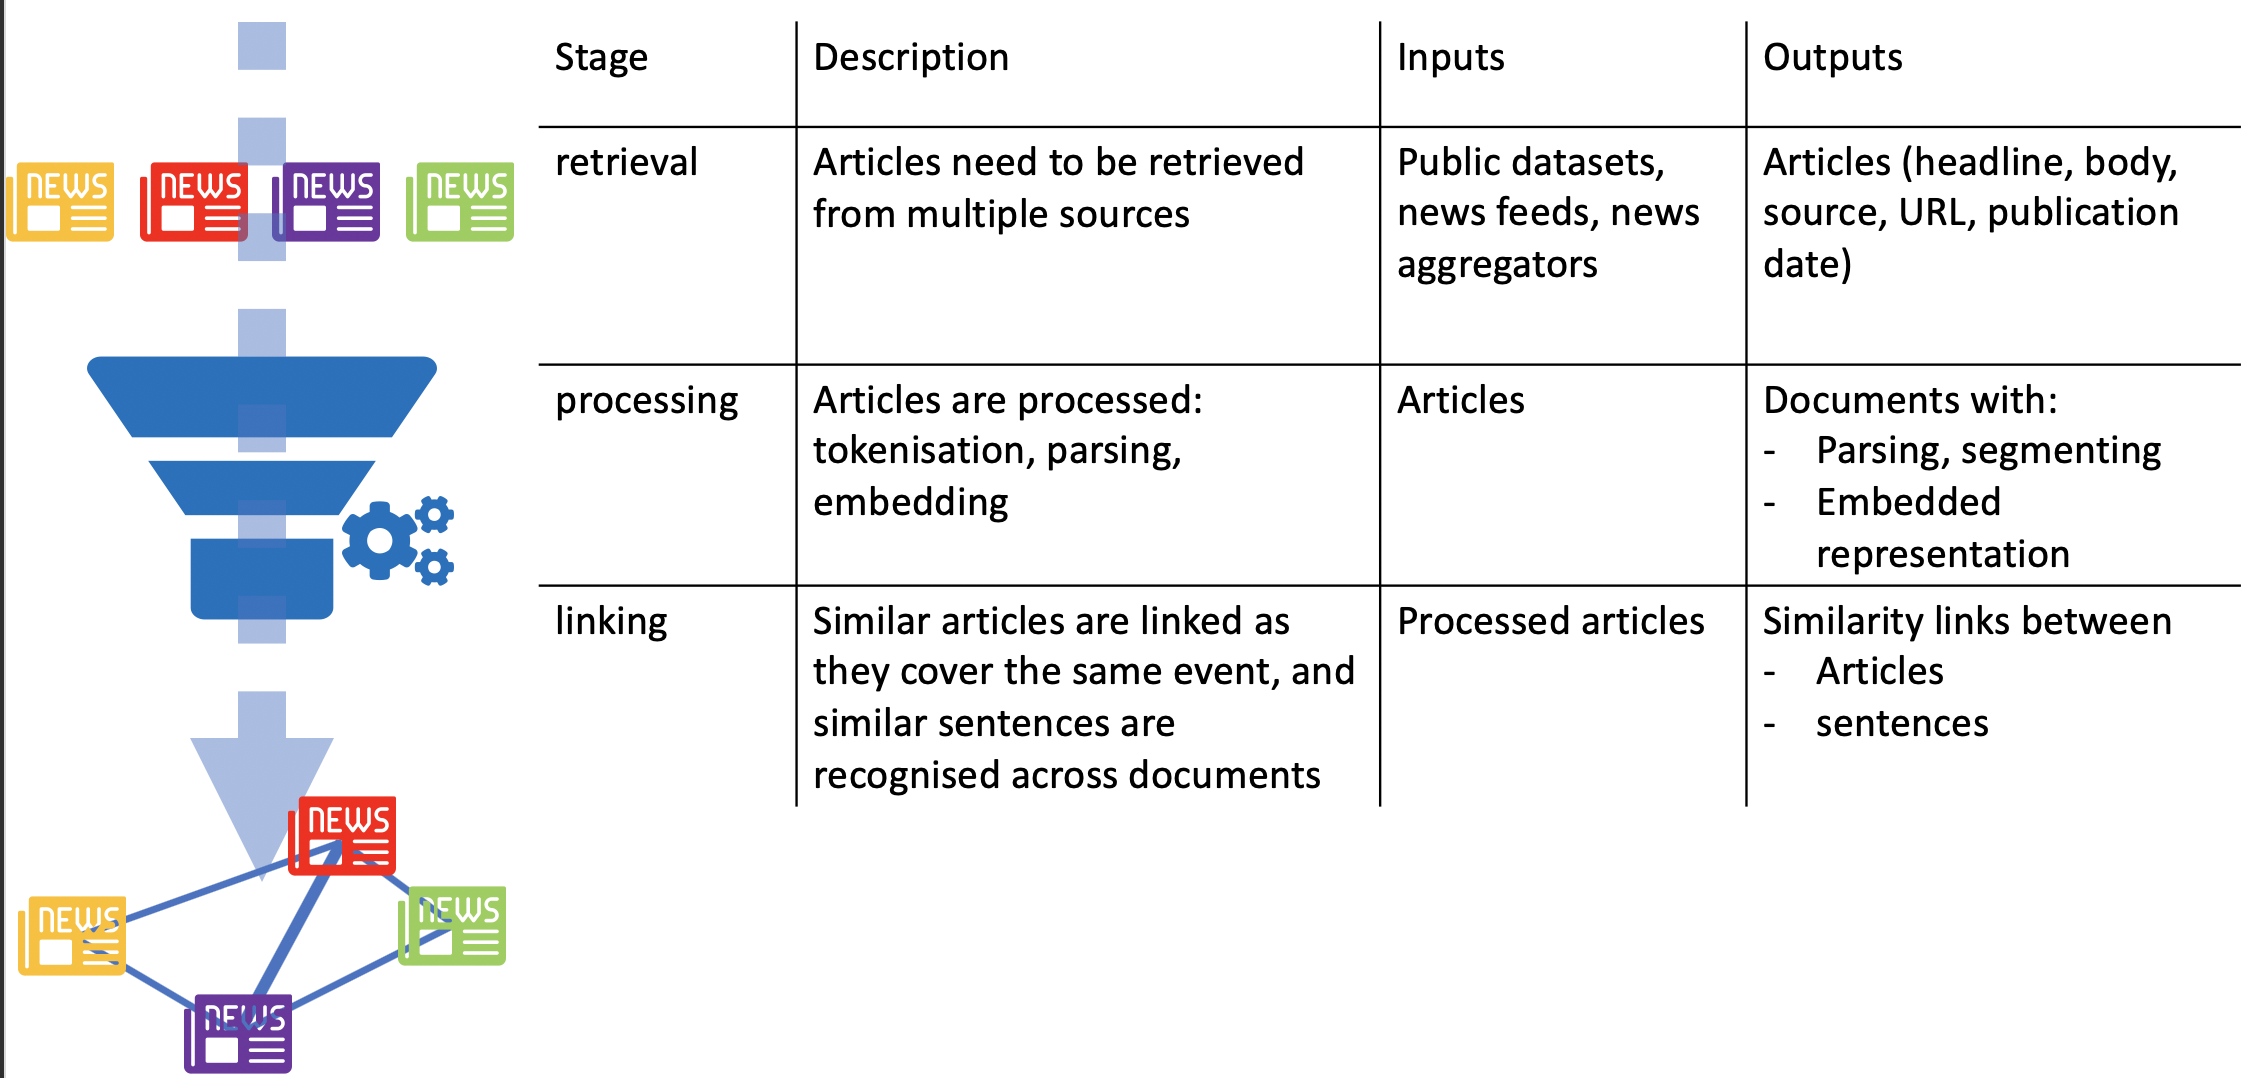
\includegraphics[width=\textwidth]{figures/figure_pipeline.png}
    \caption{The processing pipeline that retrieves, processes and links together different articles.}
    \label{fig:pipeline}
\end{figure}
\todo{redo this figure}

% hypothesis
Our hypothesis is that having the availability of multiple articles would help an automated framing detection model to find more signals of framing.
As the first sub-question analyses the importance for human readers, this analysis wants to see if it is important for the automated detection.
We also hypothesise that some types of framing signals are only detectable by using the external knowledge coming from other articles, which is not used by the existing methods.

% evaluation
To validate or refute our hypothesis, the model will be evaluated by looking at how accurately the spans containing framing differences are identified.
As a comparison, we plan to use models that instead just focus on one single article at a time to extract the features.
For example the complete model will be compared with another version (single-article) that discards the features coming from the comparison.
Or also other models found in the literature that focus on specific types of framing signals (e.g., emphasis detection, loaded terms) will be tested to see if our model (complete or incomplete) is comparable and overtakes them.
% For some of the framing signals that focus on single articles, there are baselines that are usually only available on specific topics.

% We cannot compare with mostly of them because of the different topics and because the problem

% dataset building
In order to evaluate the model proposed, we will need to collect a larger \textbf{dataset}, where manual annotators will be given the task description and will annotate on document pairs the framing differences according to the schema identified with the first user study.
% (help of pipeline to provide similar articles and candidate words/sentences based on uniqueness)
The pairs of documents will be extracted with the help of the pipeline which will provide articles that are very similar in the content but at the same time have enough differences to be annotated. % (criticality of the threshold)
The annotations will contain the type of signal and also the role/orientation of the two documents (e.g. in an omission signal, one article is \textit{including} and the other is \textit{excluding}, or instead in a term strength variation, one article is \textit{stronger} and the other is \textit{weaker}).
The annotations can be then used both in the multi-article scenario and in the single-article scenario, because different spans will be annotated on the pairs of documents.
For example, if we have an annotation that is highlighting a term that is used with a difference strength, the fact that one term is stronger is available even without having the information of the other article.
This dataset will be made available as a resource paper in order to promote the research on this task.

% outputs
Once this method has been analysed and validated, the detection model will be made available as a tool which help users to see the framing differences between multiple articles.
We plan to put it in an online setting where people will continue to provide training data by correcting or validating the outputs of the tool on new article that have not yet been analysed.
This tool will also be the founding block for the next research questions.

\subsubsection{Processing Pipeline}\todo{squeeze at the beginning of 4.1.2}
\label{sec:prop_pipeline}
The first objective is to build a representation that describes how the articles, and parts of them, are related between each other, together with the framing features coming from the single-article analysis.




As we can see in Figure~\ref{fig:pipeline}, the processing pipeline is made of different stages:
% The processing pipeline we propose for this purpose is made of multiple steps:
\begin{itemize}
    \item \textbf{preprocessing}: documents are retrieved, cleaned up and fragmented into paragraphs and sentences;
    \item \textbf{narrative features} are attached to each document, paragraph and sentence belonging to three main types:
    \emph{structural role} using and highlighting the linguistic devices provided by~\cite{zahid2019towards};
    \emph{framing features} are extracted (framing and reasoning devices) finding some linguistic representatives from~\cite{gamson1989media,fillmore2006frame};
    \emph{subjectivity} is computed, and strong word choices are highlighted~\cite{liu2010sentiment};\todo{expand on single-article framing signals}
    \item \textbf{linking}: \emph{similar articles} are found by using document-level similarity measures: in this way it would be possible to find groups of documents that describe the same events; \emph{similar sentences and paragraphs} are found by sentence-level similarity measures, inside each group of documents: corroborated and omitted sentences are identified~\cite{bountouridis2018explaining}.
\end{itemize}
% We start with an example of analysis together with the processing pipeline, % that enables this and 
% then we introduce some cross-article signals that highlight the difference in the narratives used.
% First we describe how we think is more reasonable to process the documents (similarity, cliques, hierarchical topic/stories).
% Then we describe which are the  (baseline)(with list).

At the end of the pipeline, we will have available a representation for the articles that accounts for how they are similar on the document level and at the sentence level.
% also single-article framing features
This representation would allow us to navigate between different articles and see their features. We will exploit this representation for answering the two Research Questions, as shown in the following sections.


\section{The role of news sources (RQ2)}
\label{sec:prop_rq2}
% RQ2: also the sources

The purpose of the second research question is to understand the link between the features of the sources and how they frame the news, changing details and taking information from other sources.
While the first research question focused on how to reveal the framing, here we want to investigate how the sources interact with framing. For this purpose, we have two sub-questions that investigate \emph{i)} the relationships between the features of a source and the framing that it uses, and \emph{ii)} how stories are modified and re-framed over time when sources reuse contents from other articles.

\subsection{Source features vs framing (RQ2.1)}
% RQ2.1: relationship with source information
News sources are different and there is a wide variety of them in the media landscape.
A source can have a certain political alignment, be part of a certain news group, have affiliation to certain movements and ideals, or live in a certain country, and we want to do an analysis across all these features.
% we capture all together as ``affiliation''
Lots of tools and evaluation methods just rely on the provenance of the news, looking at which source published it. The reputation of the sources is a big theme in the credibility domain.
Here we want to analyse the relationship between the features of a news source and how it applies framing differently from others. The sub-question is:
\textbf{Which features of a news source relate with the framing techniques it uses?}
We want to analyse the relationships between the framing choices done by the authors and the news sources where the articles are published. In other words, we want to understand the relationships between the ideological alignment of the news outlets (political alignment, bias, newsgroups) and the effective differences contained in the articles.


% With RQ2.1 we ask how does the framing analysis relate with the information of the single outlets (affiliation, newsgroup, bias, partisanship, ...).

% Hypothesis
The hypothesis that we have is that certain features, such as the political alignment, have bigger effects than others, especially when the news topic is about politics.
Instead for other topics we want to understand what is the effect of other features and discover which ones make the articles to be framed in a certain way.

% requirement: data on news outlets
In order to test this hypothesis we need two sets of information: the data for each of the sources and the framing analysis.
In the first group, we can use many features:

\begin{itemize}
    \item political alignment: AllSides, Media Bias/Fact Check
    \item newsgroup (TODO find)
    \item geographical information: country, region
    \item factuality rating (MBFC, NewsGuard)
    \item ideology (MBFC)
    \item 
\end{itemize}

On the other side, the framing analysis will provide how much each source uses each of the framing techniques, by doing an aggregation on the source level of the analysis of the articles.

% analysis
The analysis will be done by comparing the two sets and extracting the most important correlations.
% And once this information is available, we can aggregate a set of framing features (to be defined!!!) by the source of the articles.
\todo{describe more}

% With these two groups of information, we can study their correlation.

% possible outcomes
This correlation analysis will tell us if there are any characteristics of the news sources that make them heavily use framing techniques.
One example that we may discover is that sources heavily biased (score on the source) tend to perform omissions (as seen in~\citet{bountouridis2018explaining}) or use loaded language.


% significance


\subsection{RQ2.2}
% RQ2.2
The last sub-question instead takes the direction of analysing the evolution over time of an event in how it is presented in the media landscape.
\textbf{To what extent can we identify the evolution of the framing of a certain event?}
And if we also take the timing information (publication time), we can expand this model to characterise the evolution of information, describing how different news sources reuse contents from others and how the details are selected and changed over time.
In this way we aim to extract \textit{information flows}, showing over time how different sources treat different details of the events, evolving the narrative, acquiring new elements from other sources and dropping other information pieces.

% hypothesis
Hypothesis: We can identify patterns between certain sources that take contents from others and perform specific modifications

% requirements
Data requirements: timing information.
Is it reliable? How to manage intervals and not only instants

% analysis
\todo{describe analysis}

% outputs
\todo{describe outputs}






% Tool for finding other stories on the same event
% External facts not considered
% Highlight words that are used differently
% Tool to analyse the practices of news outlets
% From where do they get info
% How they change it
